% Capítulo 5: as três partes do for e a ordem em que são executadas.
\documentclass[border=4pt]{standalone}
\usepackage[utf8]{inputenc}
\usepackage[T1]{fontenc}
% Estilo comum dos fluxogramas e diagramas de blocos.
\usepackage{tikz}
\usetikzlibrary{arrows.meta, positioning, calc, shapes.geometric, shapes.misc}
\definecolor{navy}{RGB}{23,45,80}
\definecolor{laranja}{RGB}{250,110,29}
\definecolor{cinzalogo}{RGB}{107,114,126}
\definecolor{azul}{RGB}{205,222,247}
\tikzset{
  base/.style={draw=navy, line width=0.9pt, font=\sffamily\small, align=center, inner sep=4pt},
  terminal/.style={base, rounded rectangle, fill=laranja!45, draw=laranja, minimum width=20mm, minimum height=7mm},
  processo/.style={base, rectangle, fill=laranja!12, minimum width=28mm, minimum height=8mm},
  decisao/.style={base, diamond, aspect=2.2, fill=azul, inner sep=1pt, minimum width=30mm},
  es/.style={base, trapezium, trapezium left angle=72, trapezium right angle=108,
             fill=white, minimum width=26mm, minimum height=8mm, trapezium stretches body},
  fluxo/.style={-{Stealth[length=2.2mm]}, navy, line width=0.9pt},
  rotulo/.style={font=\sffamily\small\bfseries, text=navy},
  legenda/.style={font=\sffamily\scriptsize, text=cinzalogo},
  resposta/.style={font=\sffamily\scriptsize\bfseries, text=navy},
}

\tikzset{
  parte/.style={rounded corners=2pt, inner sep=2pt, font=\ttfamily\small},
  num/.style={circle, fill=laranja, text=white, font=\sffamily\scriptsize\bfseries, inner sep=0pt, minimum size=4.2mm},
  expl/.style={font=\sffamily\scriptsize, text=navy, align=center},
  guia/.style={draw=cinzalogo, line width=0.5pt},
}
\begin{document}
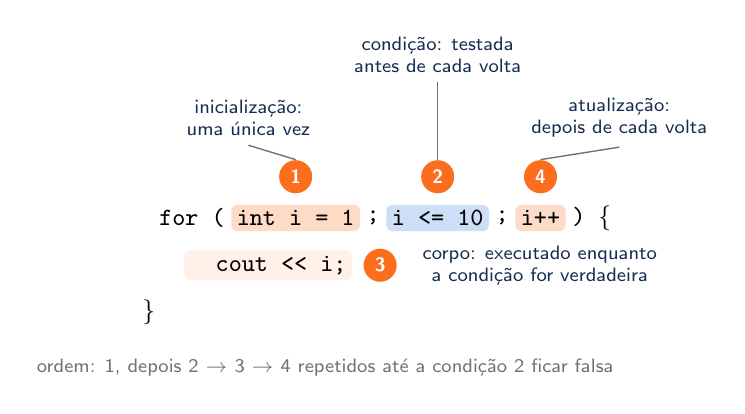
\begin{tikzpicture}
  \node[parte, anchor=east] (f) at (0, 0) {for (};
  \node[parte, fill=laranja!25, anchor=west] (ini) at (f.east) {int i = 1};
  \node[parte, anchor=west] (p1) at (ini.east) {;};
  \node[parte, fill=azul, anchor=west] (cond) at (p1.east) {i <= 10};
  \node[parte, anchor=west] (p2) at (cond.east) {;};
  \node[parte, fill=laranja!25, anchor=west] (atu) at (p2.east) {i++};
  \node[parte, anchor=west] (p3) at (atu.east) {) \{};
  \node[parte, fill=laranja!10, anchor=west] (corpo) at (-0.6, -0.6) {\quad cout <{}< i;};
  \node[parte, anchor=west] at (-1.2, -1.2) {\}};

  \node[num] (n1) at ($(ini.north)+(0, 0.35)$) {1};
  \node[num] (n2) at ($(cond.north)+(0, 0.35)$) {2};
  \node[num] (n3) at ($(corpo.east)+(0.35, 0)$) {3};
  \node[num] (n4) at ($(atu.north)+(0, 0.35)$) {4};

  \node[expl] (e1) at ($(ini.north)+(-0.6, 1.1)$) {inicialização:\\uma única vez};
  \node[expl] (e2) at ($(cond.north)+(0, 1.9)$) {condição: testada\\antes de cada volta};
  \node[expl] (e4) at ($(atu.north)+(1.0, 1.1)$) {atualização:\\depois de cada volta};
  \draw[guia] (e1.south) -- (n1.north);
  \draw[guia] (e2.south) -- (n2.north);
  \draw[guia] (e4.south) -- (n4.north);
  \node[expl, anchor=west] at ($(n3.east)+(0.2, 0)$) {corpo: executado enquanto\\a condição for verdadeira};
  \node[legenda] at (1.2, -1.9) {ordem: 1, depois 2 $\rightarrow$ 3 $\rightarrow$ 4 repetidos até a condição 2 ficar falsa};
\end{tikzpicture}
\end{document}
